% Options for packages loaded elsewhere
\PassOptionsToPackage{unicode}{hyperref}
\PassOptionsToPackage{hyphens}{url}
\PassOptionsToPackage{dvipsnames,svgnames,x11names}{xcolor}
%
\documentclass[
  article]{jss}

\usepackage{amsmath,amssymb}
\usepackage{iftex}
\ifPDFTeX
  \usepackage[T1]{fontenc}
  \usepackage[utf8]{inputenc}
  \usepackage{textcomp} % provide euro and other symbols
\else % if luatex or xetex
  \usepackage{unicode-math}
  \defaultfontfeatures{Scale=MatchLowercase}
  \defaultfontfeatures[\rmfamily]{Ligatures=TeX,Scale=1}
\fi
\usepackage{lmodern}
\ifPDFTeX\else  
    % xetex/luatex font selection
\fi
% Use upquote if available, for straight quotes in verbatim environments
\IfFileExists{upquote.sty}{\usepackage{upquote}}{}
\IfFileExists{microtype.sty}{% use microtype if available
  \usepackage[]{microtype}
  \UseMicrotypeSet[protrusion]{basicmath} % disable protrusion for tt fonts
}{}
\makeatletter
\@ifundefined{KOMAClassName}{% if non-KOMA class
  \IfFileExists{parskip.sty}{%
    \usepackage{parskip}
  }{% else
    \setlength{\parindent}{0pt}
    \setlength{\parskip}{6pt plus 2pt minus 1pt}}
}{% if KOMA class
  \KOMAoptions{parskip=half}}
\makeatother
\usepackage{xcolor}
\setlength{\emergencystretch}{3em} % prevent overfull lines
\setcounter{secnumdepth}{-\maxdimen} % remove section numbering
% Make \paragraph and \subparagraph free-standing
\ifx\paragraph\undefined\else
  \let\oldparagraph\paragraph
  \renewcommand{\paragraph}[1]{\oldparagraph{#1}\mbox{}}
\fi
\ifx\subparagraph\undefined\else
  \let\oldsubparagraph\subparagraph
  \renewcommand{\subparagraph}[1]{\oldsubparagraph{#1}\mbox{}}
\fi


\providecommand{\tightlist}{%
  \setlength{\itemsep}{0pt}\setlength{\parskip}{0pt}}\usepackage{longtable,booktabs,array}
\usepackage{calc} % for calculating minipage widths
% Correct order of tables after \paragraph or \subparagraph
\usepackage{etoolbox}
\makeatletter
\patchcmd\longtable{\par}{\if@noskipsec\mbox{}\fi\par}{}{}
\makeatother
% Allow footnotes in longtable head/foot
\IfFileExists{footnotehyper.sty}{\usepackage{footnotehyper}}{\usepackage{footnote}}
\makesavenoteenv{longtable}
\usepackage{graphicx}
\makeatletter
\def\maxwidth{\ifdim\Gin@nat@width>\linewidth\linewidth\else\Gin@nat@width\fi}
\def\maxheight{\ifdim\Gin@nat@height>\textheight\textheight\else\Gin@nat@height\fi}
\makeatother
% Scale images if necessary, so that they will not overflow the page
% margins by default, and it is still possible to overwrite the defaults
% using explicit options in \includegraphics[width, height, ...]{}
\setkeys{Gin}{width=\maxwidth,height=\maxheight,keepaspectratio}
% Set default figure placement to htbp
\makeatletter
\def\fps@figure{htbp}
\makeatother

\usepackage{orcidlink,thumbpdf,lmodern}

\newcommand{\class}[1]{`\code{#1}'}
\newcommand{\fct}[1]{\code{#1()}}
\makeatletter
\@ifpackageloaded{tcolorbox}{}{\usepackage[skins,breakable]{tcolorbox}}
\@ifpackageloaded{fontawesome5}{}{\usepackage{fontawesome5}}
\definecolor{quarto-callout-color}{HTML}{909090}
\definecolor{quarto-callout-note-color}{HTML}{0758E5}
\definecolor{quarto-callout-important-color}{HTML}{CC1914}
\definecolor{quarto-callout-warning-color}{HTML}{EB9113}
\definecolor{quarto-callout-tip-color}{HTML}{00A047}
\definecolor{quarto-callout-caution-color}{HTML}{FC5300}
\definecolor{quarto-callout-color-frame}{HTML}{acacac}
\definecolor{quarto-callout-note-color-frame}{HTML}{4582ec}
\definecolor{quarto-callout-important-color-frame}{HTML}{d9534f}
\definecolor{quarto-callout-warning-color-frame}{HTML}{f0ad4e}
\definecolor{quarto-callout-tip-color-frame}{HTML}{02b875}
\definecolor{quarto-callout-caution-color-frame}{HTML}{fd7e14}
\makeatother
\makeatletter
\makeatother
\makeatletter
\makeatother
\makeatletter
\@ifpackageloaded{caption}{}{\usepackage{caption}}
\AtBeginDocument{%
\ifdefined\contentsname
  \renewcommand*\contentsname{Table of contents}
\else
  \newcommand\contentsname{Table of contents}
\fi
\ifdefined\listfigurename
  \renewcommand*\listfigurename{List of Figures}
\else
  \newcommand\listfigurename{List of Figures}
\fi
\ifdefined\listtablename
  \renewcommand*\listtablename{List of Tables}
\else
  \newcommand\listtablename{List of Tables}
\fi
\ifdefined\figurename
  \renewcommand*\figurename{Figure}
\else
  \newcommand\figurename{Figure}
\fi
\ifdefined\tablename
  \renewcommand*\tablename{Table}
\else
  \newcommand\tablename{Table}
\fi
}
\@ifpackageloaded{float}{}{\usepackage{float}}
\floatstyle{ruled}
\@ifundefined{c@chapter}{\newfloat{codelisting}{h}{lop}}{\newfloat{codelisting}{h}{lop}[chapter]}
\floatname{codelisting}{Listing}
\newcommand*\listoflistings{\listof{codelisting}{List of Listings}}
\makeatother
\makeatletter
\@ifpackageloaded{caption}{}{\usepackage{caption}}
\@ifpackageloaded{subcaption}{}{\usepackage{subcaption}}
\makeatother
\makeatletter
\makeatother
\ifLuaTeX
  \usepackage{selnolig}  % disable illegal ligatures
\fi
\IfFileExists{bookmark.sty}{\usepackage{bookmark}}{\usepackage{hyperref}}
\IfFileExists{xurl.sty}{\usepackage{xurl}}{} % add URL line breaks if available
\urlstyle{same} % disable monospaced font for URLs
\hypersetup{
  pdftitle={Making, Updating, and Querying Causal Models using CausalQueries},
  pdfauthor={Till Tietz; Lily Medina; Macartan Humphreys},
  pdfkeywords={causal models, stan, bayes},
  colorlinks=true,
  linkcolor={blue},
  filecolor={Maroon},
  citecolor={Blue},
  urlcolor={Blue},
  pdfcreator={LaTeX via pandoc}}

%% -- Article metainformation (author, title, ...) -----------------------------

%% Author information
\author{Till Tietz\\WZB \And Lily Medina\\UC Berkeley \AND Macartan
Humphreys~\orcidlink{0000-0001-7029-2326}\\WZB}
\Plainauthor{Till Tietz, Lily Medina, Macartan
Humphreys} %% comma-separated

\title{Making, Updating, and Querying Causal Models using
\texttt{CausalQueries}}
\Plaintitle{Making, Updating, and Querying Causal Models using
CausalQueries} %% without formatting

%% an abstract and keywords
\Abstract{A guide to the \proglang{R} package \texttt{CausalQueries} for
making, updating, and querying causal models}

%% at least one keyword must be supplied
\Keywords{causal models, stan, bayes}
\Plainkeywords{causal models, stan, bayes}

%% publication information
%% NOTE: Typically, this can be left commented and will be filled out by the technical editor
%% \Volume{50}
%% \Issue{9}
%% \Month{June}
%% \Year{2012}
%% \Submitdate{2012-06-04}
%% \Acceptdate{2012-06-04}
%% \setcounter{page}{1}
%% \Pages{1--xx}

%% The address of (at least) one author should be given
%% in the following format:
\Address{
Till Tietz\\
IPI\\
Reichpietschufer 50\\
Berlin Germany\\
E-mail: \email{ttietz2014@gmail.com}\\
\\~
Lily Medina\\
\\~
Macartan Humphreys\\
E-mail: \email{macartan.humphreys@wzb.eu}\\
URL: \url{https://macartan.github.io/}\\
\\~

}

\begin{document}
\maketitle
\hypertarget{sec-intro}{%
\section{Introduction: Causal models}\label{sec-intro}}

\begin{itemize}
\tightlist
\item
  Embed the \emph{methods} and the \emph{software} into the respective
  relevant literature.
\item
  For the latter both competing and complementary software should be
  discussed (within the same software environment and beyond), bringing
  out relative (dis)advantages. All software mentioned should be
  properly \texttt{@cited}'d.~(See also
  \protect\hyperlink{sec-bibtex}{Using BibTeX} for more details on
  \textsc{Bib}{\TeX}.)
\end{itemize}

Leadning about causal models\ldots{}

In \proglang{R}, \ldots{}

The strength of \texttt{CausalQueries} The limitation of
\texttt{CausalQueries}

\hypertarget{sec-models}{%
\section{Models and software}\label{sec-models}}

Nodes and nodal types

\hypertarget{making-models}{%
\section{Making models}\label{making-models}}

Simple illustration

\begin{verbatim}
R> model <- make_model("Z -> X -> Y <-> X")
\end{verbatim}

\hypertarget{graphing}{%
\subsection{Graphing}\label{graphing}}

Once defined the model can be plotted:

\begin{figure}

{\centering 

\begin{verbatim}
model |> plot()
\end{verbatim}

\begin{figure}[H]

{\centering 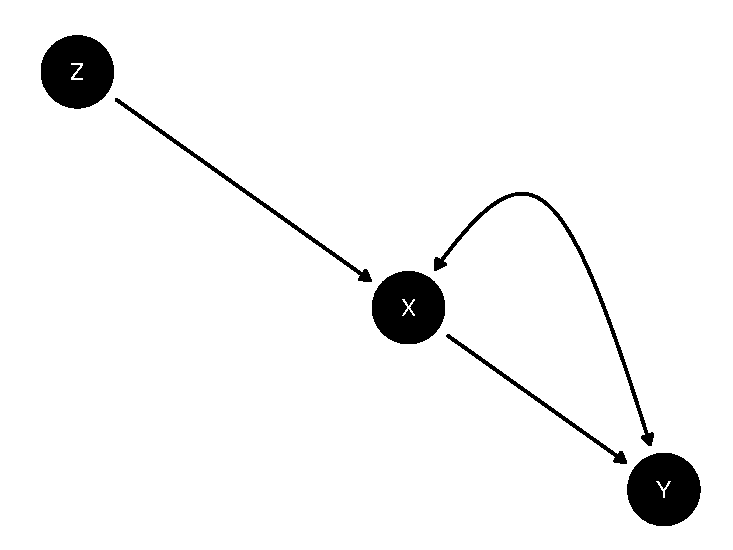
\includegraphics{paper_files/figure-pdf/unnamed-chunk-3-1.pdf}

}

\caption{A simple DAG}

\end{figure}

}

\caption{\label{fig-dag}\textbf{?(caption)}}

\end{figure}

\hypertarget{drawing-data}{%
\subsection{Drawing data}\label{drawing-data}}

\begin{verbatim}
model |> make_data(n = 5) |> kable()
\end{verbatim}

\begin{longtable}[]{@{}rrr@{}}
\toprule\noalign{}
Z & X & Y \\
\midrule\noalign{}
\endhead
\bottomrule\noalign{}
\endlastfoot
0 & 1 & 0 \\
0 & 1 & 0 \\
0 & 1 & 1 \\
1 & 1 & 0 \\
1 & 1 & 1 \\
\end{longtable}

\hypertarget{updating-models}{%
\section{Updating models}\label{updating-models}}

\hypertarget{the-stan-model}{%
\subsection{The stan model}\label{the-stan-model}}

As \texttt{update\_model()} calls \texttt{rstan::sampling} one can pass
along all arguments in \texttt{...} to \texttt{rstan::sampling}.

\hypertarget{stan-data}{%
\subsection{stan data}\label{stan-data}}

\hypertarget{censored-data}{%
\subsection{censored data}\label{censored-data}}

\hypertarget{output}{%
\subsection{Output}\label{output}}

The primary output from \texttt{update\_model()} is a posterior
distribution over model parameters, stored as a dataframe in
\texttt{model\$posterior\_distribution}. However another of other
objects are also optionally stored:

\hypertarget{querying-models}{%
\section{Querying models}\label{querying-models}}

\hypertarget{querying-distributions}{%
\subsection{Querying distributions}\label{querying-distributions}}

\hypertarget{case-level-queries}{%
\subsection{Case level queries}\label{case-level-queries}}

\hypertarget{illustrations}{%
\section{Illustrations}\label{illustrations}}

\hypertarget{identification-with-causalqueries}{%
\subsection{Identification with
CausalQueries}\label{identification-with-causalqueries}}

\hypertarget{computational-details}{%
\section*{Computational details}\label{computational-details}}
\addcontentsline{toc}{section}{Computational details}

\begin{itemize}
\tightlist
\item
  information about certain computational details such as version
  numbers, operating systems, or compilers could be included in an
  unnumbered section. Also, auxiliary packages (say, for visualizations,
  maps, tables, \ldots) that are not cited in the main text can be
  credited here.
\end{itemize}

:::

The results in this paper were obtained using
\proglang{R}\textasciitilde3.4.1 with the
\pkg{MASS}\textasciitilde7.3.47 package. \proglang{R} itself and all
packages used are available from the Comprehensive \proglang{R} Archive
Network (CRAN) at {[}https://CRAN.R-project.org/{]}.

\hypertarget{acknowledgments}{%
\section*{Acknowledgments}\label{acknowledgments}}
\addcontentsline{toc}{section}{Acknowledgments}

\begin{tcolorbox}[enhanced jigsaw, rightrule=.15mm, opacityback=0, breakable, arc=.35mm, left=2mm, toprule=.15mm, bottomrule=.15mm, colback=white, leftrule=.75mm]

All acknowledgments (note the AE spelling) should be collected in this
unnumbered section before the references. It may contain the usual
information about funding and feedback from colleagues/reviewers/etc.
Furthermore, information such as relative contributions of the authors
may be added here (if any).

\end{tcolorbox}

\hypertarget{references}{%
\section*{References}\label{references}}
\addcontentsline{toc}{section}{References}

\renewcommand{\bibsection}{}
\bibliography{bibliography.bib}

\newpage{}

\hypertarget{sec-techdetails}{%
\section*{More technical details}\label{sec-techdetails}}
\addcontentsline{toc}{section}{More technical details}

\begin{tcolorbox}[enhanced jigsaw, rightrule=.15mm, opacityback=0, breakable, arc=.35mm, left=2mm, toprule=.15mm, bottomrule=.15mm, colback=white, leftrule=.75mm]

Appendices can be included after the bibliography (with a page break).
Each section within the appendix should have a proper section title
(rather than just \emph{Appendix}).

For more technical style details, please check out JSS's style FAQ at
{[}https://www.jstatsoft.org/pages/view/style\#frequently-asked-questions{]}
which includes the following topics:

\begin{itemize}
\tightlist
\item
  Title vs.~sentence case.
\item
  Graphics formatting.
\item
  Naming conventions.
\item
  Turning JSS manuscripts into \proglang{R} package vignettes.
\item
  Trouble shooting.
\item
  Many other potentially helpful details\ldots{}
\end{itemize}

\end{tcolorbox}

\hypertarget{sec-bibtex}{%
\section*{Using BibTeX}\label{sec-bibtex}}
\addcontentsline{toc}{section}{Using BibTeX}

\begin{tcolorbox}[enhanced jigsaw, rightrule=.15mm, opacityback=0, breakable, arc=.35mm, left=2mm, toprule=.15mm, bottomrule=.15mm, colback=white, leftrule=.75mm]

References need to be provided in a \textsc{Bib}{\TeX} file
(\texttt{.bib}). All references should be made with \texttt{@cite}
syntax. This commands yield different formats of author-year citations
and allow to include additional details (e.g.,pages, chapters, \dots) in
brackets. In case you are not familiar with these commands see the JSS
style FAQ for details.

Cleaning up \textsc{Bib}{\TeX} files is a somewhat tedious task --
especially when acquiring the entries automatically from mixed online
sources. However, it is important that informations are complete and
presented in a consistent style to avoid confusions. JSS requires the
following format.

\begin{itemize}
\tightlist
\item
  item JSS-specific markup (\texttt{\textbackslash{}proglang},
  \texttt{\textbackslash{}pkg}, \texttt{\textbackslash{}code}) should be
  used in the references.
\item
  item Titles should be in title case.
\item
  item Journal titles should not be abbreviated and in title case.
\item
  item DOIs should be included where available.
\item
  item Software should be properly cited as well. For \proglang{R}
  packages \texttt{citation("pkgname")} typically provides a good
  starting point.
\end{itemize}

\end{tcolorbox}




\end{document}
